\chapter{Base de données}

\section{Qu'est-ce qu'un base de données ?}

Une \emph{base de données} est un moyen de stocker, d'organiser et de hiérarchiser des données. Une base de données peut être rapprochée d'un classeur Calc ou Microsoft Excel :
\begin{itemize}
	\item chaque fichier est une base de données ;
	\item chaque onglet (feuille) correspond à une table ;
	\item chaque colonne (ou ligne) est un champ spécifiant une caractéristique des données ;
	\item chaque ligne (ou colonne) est un enregistrement, une donnée.
\end{itemize}

\Espace

Il existe plusieurs moyens de stocker des données.
\begin{itemize}
	\item Le format texte (\verb-.txt-) est un choix assez évident pour les néophytes, il ne nécessite pas de logiciels supplémentaires. Mais, il est peu efficace, un fichier devient vite encombrant, il utilise beaucoup de ressources à la lecture et à l'écriture, et chaque table nécessite un fichier séparé qui est ouvert tour-à-tour.
	
	\item Le format texte optimisé pour les données (\verb-.csv-) ne nécessite pas de logiciels supplémentaires. C'est un moyen efficace de stocker les données quand il est bien utilisé. Mais, il a les mêmes inconvénients que le format texte.
	
	\item Le classeur Excel ou Calc (\verb-.xls-, \verb-.xlsx- ou \verb-.ods-) est équivalent à une base de données. Mais, le fichier devient encombrant et est peu pratique à utiliser, il consomme beaucoup de ressources, il n'est pas optimisé pour être utilisé sur un serveur et il doit être créé par un logiciel externe.
	
	\item Le format Microsoft DataBase (\verb-.mdb-) est un format spécial base de données, il est entièrement fonctionnel sous Windows. Mais, il est impossible à utiliser avec des outils gratuits et doit être créé par un logiciel externe.
	
	\item Le format OpenDocument Database (\verb-.odb-) est un format de bases de données libre. Mais, tout comme le précédent, il doit être créé par un logiciel extérieur
	
	\item Enfin, le format SQL (\emph{Structured Query Language} en anglais, \verb-.sql-) est gratuit et libre. Il est issu d'un consensus entre les différentes technologies pour unifier leur utilisation. Sa connexion est simple (selon les systèmes) ainsi que les requêtes basiques mais peuvent êtres complexes suivant les besoins. Mais, il nécessite un Système de Gestion de Base de Données (ou SGBD) comme PostrgeSQL, MySQL ou ORACLE qu'il faut installer.
\end{itemize}

\section{Notre utilisation}

Afin de stocker les différentes données acquises par la partie électronique, nous devons utiliser une base de données avec un champs pour le temps, la température et la pression.

\Espace

Pour notre site, nous utilisons MySQL, un Système de Gestion de Base de Données Relationnel (SGBDR) qui peut créer et gérer des relations entre différentes tables, couplé avec le module PDO de PHP pour se connecter à la base.

Pour pouvoir utiliser une base de données, il faut d'abord installer le serveur MySQL, dont l'installation sera détaillée dans la section \ref{section:logiciels}.

Après l'installation, nous devons créer la base (que l'on nommera \verb-tpe-). Pour ce faire, dans la console MySQL ou \emph{via} phpMyAdmin (administation pour MySQL en ligne), nous rentrerons le requête suivante :
\FichierCode{SQL}{Codes/SQL/Creation_BDD.sql}

La base est alors créée mais encore inutilisable car ne contenant pas de tables. Nous créons donc une table nommée \verb-datalog_meteo- contenant plusieurs champs avec la requête:
\FichierCode{SQL}{Codes/SQL/Creation_table.sql}
La requête crée une table avec les champs \verb-id- (une valeur qui s'auto-incrémente pour différencier les enregistrements), \verb-temps- (une valeur de temps), \verb-temperature- (un nombre décimal) et \verb-pression- (un nombre décimal également). 

\begin{figure}[!h]
	\centering
	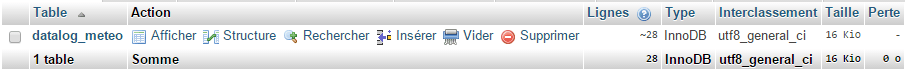
\includegraphics[width=.8\linewidth]{Images/BDD}
	
	\vspace{5mm}
	
	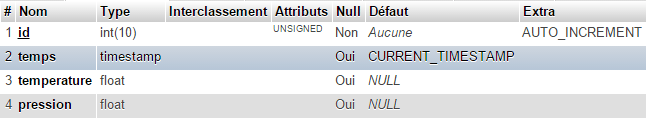
\includegraphics[width=.8\linewidth]{Images/Structure_BDD}
	\caption{Structure de notre base}
\end{figure}

La table est bien créée et utilisable mais est vide. Pour la remplir, nous utilisons la requête :
\FichierCode{SQL}{Codes/SQL/Donnees_table.sql}
La requête \verb-INSERT INTO (table) (champs)- indique à MySQL qu'il doit insérer dans les champs indiqués de la table les valeurs suivant le mot-clé \verb-VALUES-.

Nous pouvons maintenant afficher les valeurs contenues dans la table grâce à la requête:
\FichierCode{SQL}{Codes/SQL/Afficher_BDD.sql}

Cette requête affiche tout le contenu de la table \verb-datalog_meteo- sans exception. Nous pouvons cependant restreindre celui-ci en donnant les noms des champs nous étant utile, et, par exemple, un intervalle de temps ou une limite (une limite de $x$ valeurs retournera au plus $x$ valeurs).

Nous utiliserons par défaut les 20 dernières valeurs, la requête la plus utilisée est alors 
\FichierCode{SQL}{Codes/SQL/Limit_BDD.sql}
Nous demandons au serveur SQL de renvoyer les valeurs des champs \verb-temps-, \verb-temperature- et \verb-pression- dans l'ordre de temps décroissant et dans la limite de 20 valeurs. Le serveur renvoie alors un ensemble de données ressemblant à la figure suivante (dépendant des données).

\begin{figure}[!h]
	\centering
	\begin{minipage}{.5\linewidth}
		\centering
		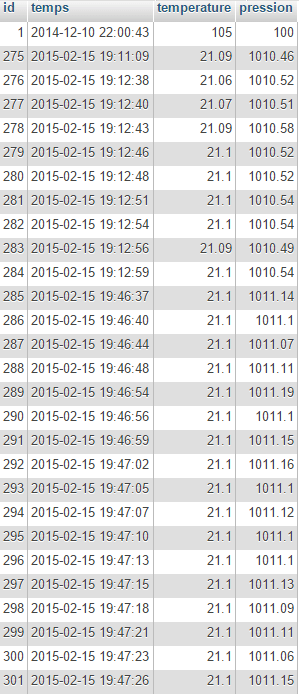
\includegraphics[width=.8\linewidth]{Images/Donnees_BDD}
	\end{minipage}%
	\begin{minipage}{.5\linewidth}
		\centering
		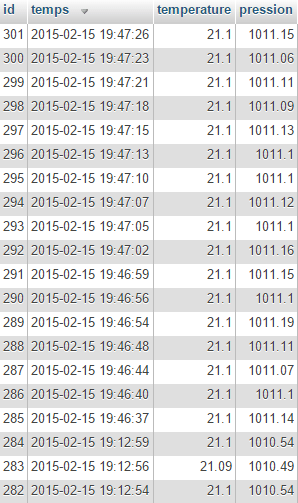
\includegraphics[width=.8\linewidth]{Images/Limit_BDD}
	\end{minipage}
	\cprotect\caption{Données de la base sans et avec \verb-LIMIT-}
\end{figure}